%============================ MAIN DOCU =================================
% define document class
\PassOptionsToPackage{table}{xcolor}
\documentclass[
    invert-title=false,
    titlepage=true,
    titleimage-ratio=1011,
    parskip=half-,
]{bfhpub}                % KOMA-script report
%---------------------------------------------------------------------------
%-----------------  Base packages     --------------------------------------
% Include Packages
\usepackage[french,ngerman,main=english]{babel}
%---------------------------------------------------------------------------
% Hyperref Package (Create links in a pdf)
%---------------------------------------------------------------------------
\usepackage[
    hidelinks
,colorlinks
,linkcolor=.
,filecolor=BFH-MediumGreen
,urlcolor=BFH-MediumBlue
,plainpages=false
,pdfpagelabels
,pdfusetitle
,hypertexnames = {true},    % no failures "same page(i)"
]{hyperref}

\usepackage{geometry}
%\usepackage[showframe]{geometry}
\usepackage{multicol}
\usepackage{graphicx}
\usepackage{caption}

%-----------------  Bibliography---   --------------------------------------
\usepackage[
    backend=biber,
    style=ieee,
    sorting=ynt
]{biblatex}
\addbibresource{body_language.bib}

%-----------------  Custom commands   --------------------------------------
% to retrieve the doc title using THETITLE
\newcommand*{\pkg}[1]{\texttt{#1}}
\newcommand*{\cls}[1]{\texttt{#1}}
\newcommand*{\code}[1]{\texttt{#1}}

%-----------------  Style and layout  --------------------------------------
\KOMAoptions{headsepline,plainheadsepline,footsepline,plainfootsepline}% add seperator line
\setkomafont{pagenumber}{\color{BFH-DarkBlue}}
\setkomafont{headsepline}{\color{BFH-DarkBlue}} % BFH-DarkBlue requires bfhcolors package
\setkomafont{footsepline}{\color{BFH-DarkBlue}} %
\chead*{Kommunikation 1 für die Informatik: Körpersprache}
\setlength\parindent{12pt}
\LoadBFHModule{boxes,tabular}
\captionsetup{
    justification = centering
}
%----------------  BFH tile page   -----------------------------------------
\title{Körpersprache}
\subtitle{Kommunikation 1 für die Informatik - Prof. Thomas von Burg - HS 2022}
\author{Fabio Bertagna}
%  \publishers{publishers}
\institution{Bern University of Applied Sciences}
\department{Technik und Informatik}
\institute{Kommunikation 1 für die Informatik}
%The starred variant will automatically scale and clip the image. the non-starred one will allow you to set the size yourself
\titlegraphic*{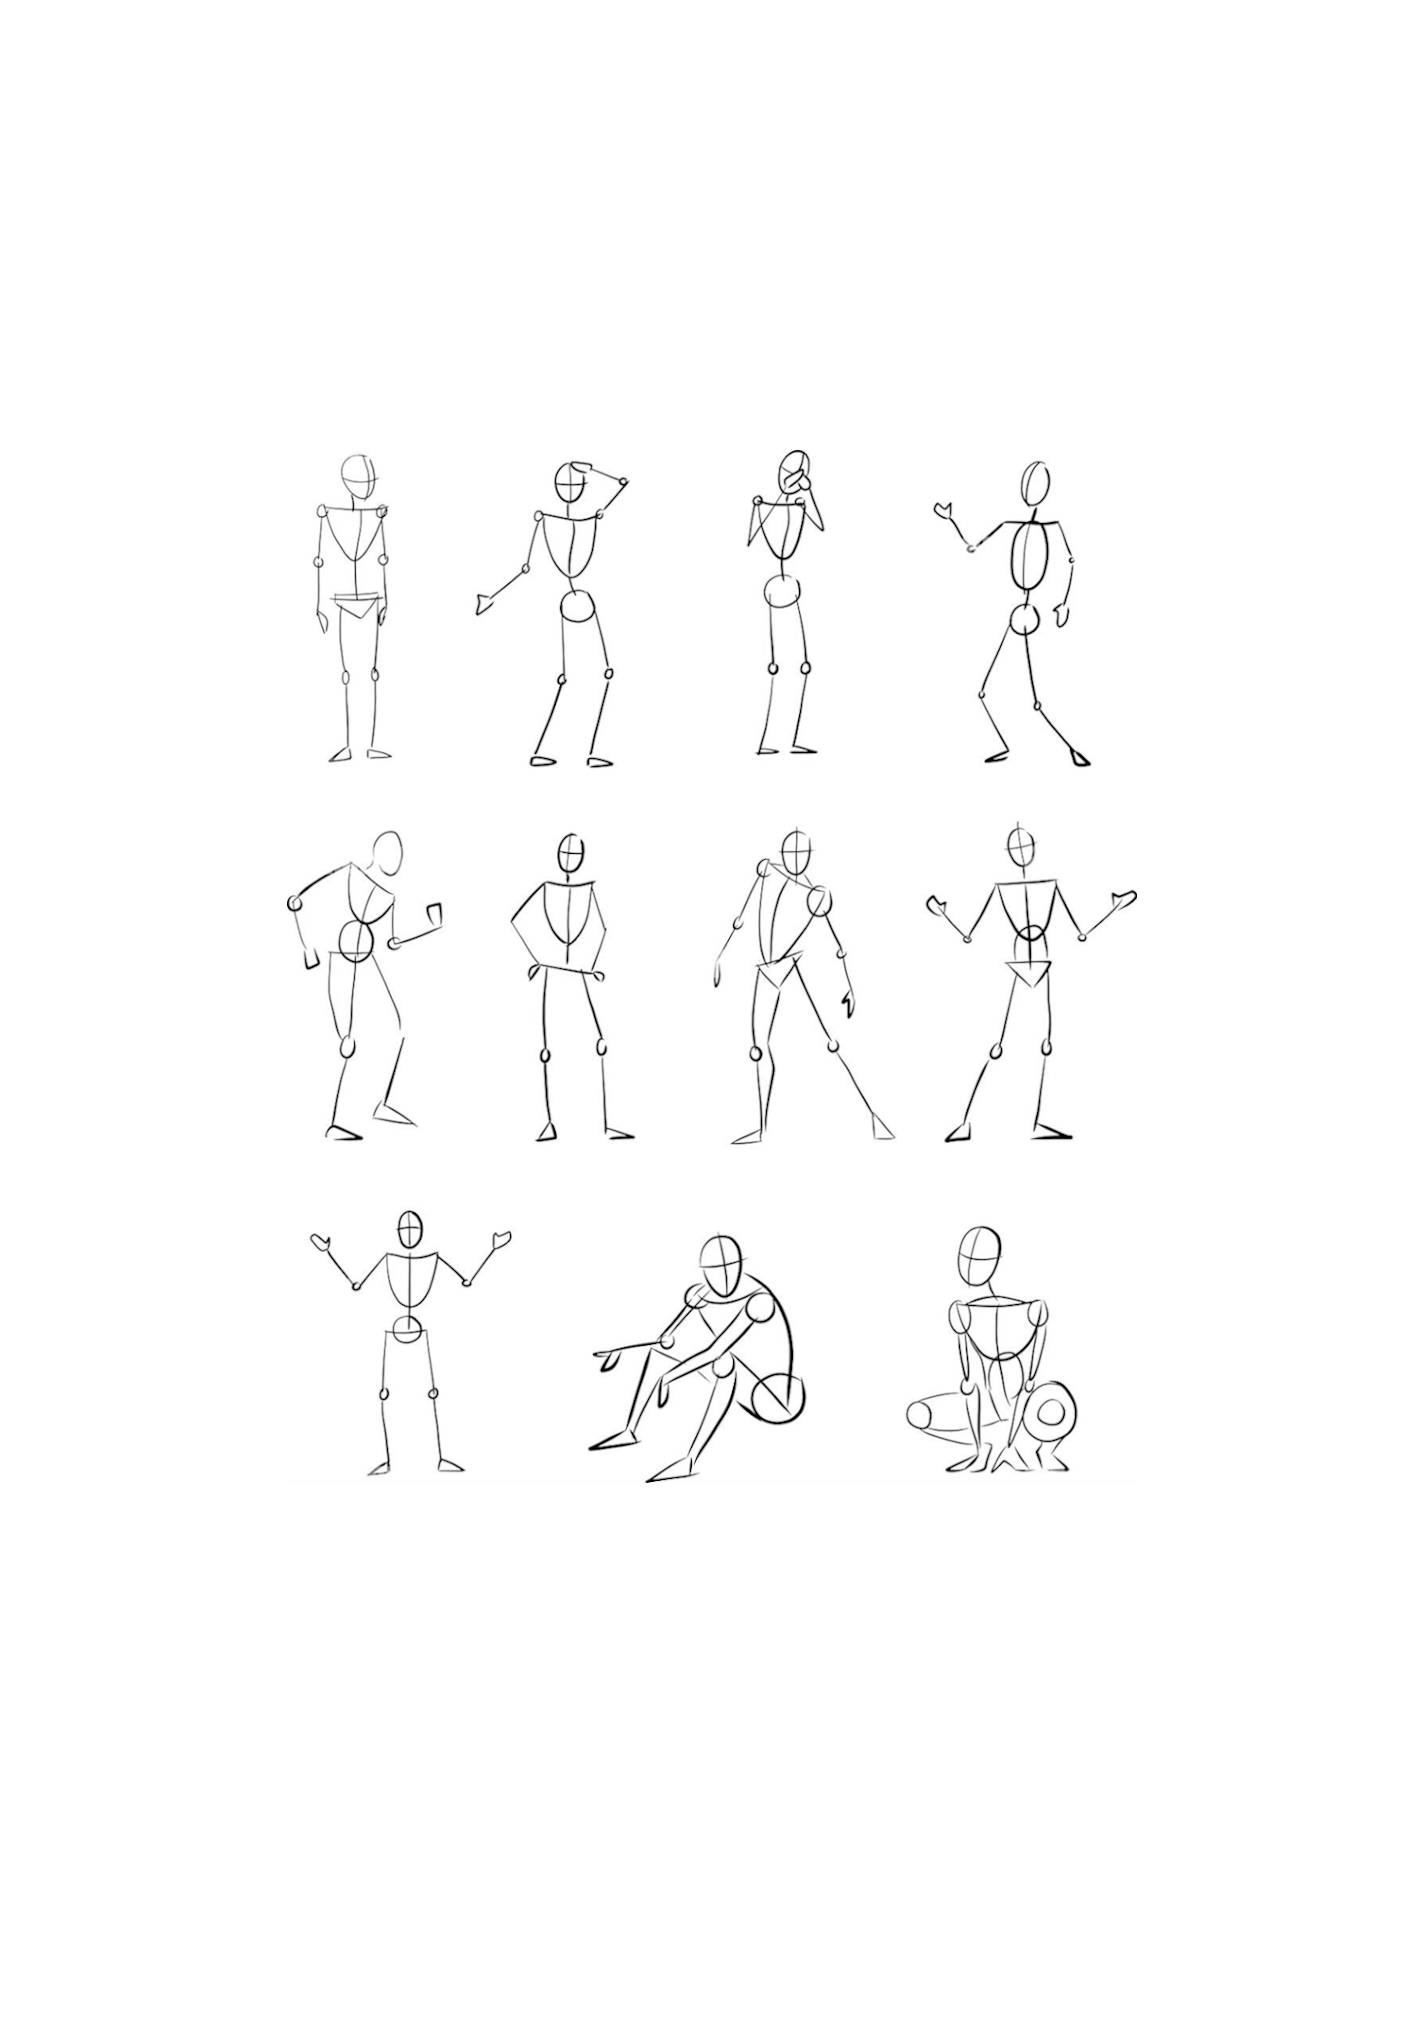
\includegraphics{images/title_page}}


\begin{document}

    \maketitle
%------------ TABLEOFCONTENTS ---------------
    \tableofcontents

    \section{Einleitung}\label{sec:vorwort}
Noch bevor wir unsere erste Sprache erlernen, besitzen wir die Fähigkeit uns ganz ohne Worte zu verständigen.
Ob ein Säugling durch sein Weinen uns seine Unzufriedenheit mitteilt,
oder ein Fussballspieler mit erhobenen Armen sein Tor zelebriert,
wir Menschen besitzen die Fähigkeit solche universell verständlichen Kommunikationsweisen zu deuten.
Diese Arbeit analysiert diese Art von Kommunikation, oft als Körpersprache bezeichnet, auf ihre theoretischen Bausteine,
zeigt auf wie wir unser Umfeld bewusster deuten können und wie wir mit der eigenen Körpersprache unser Umfeld beeinflussen können.
\par
Der Inhalt dieser Arbeit basiert auf zwei Bücher geschrieben von Joe Navarro über die menschliche Körpersprache,
welche theoretischen Aufschluss wie auch praktische Ratschläge geben,
wie wir in unserem privaten wie auch im geschäftlichen Leben unser Umfeld deuten und beeinflussen können.\cite{menschen_verstehen_und_lenken,menschen_lesen}

    \include{content/behagen_unbehagen}

    \section{Das dreieinige Gehirn}\label{sec:das-dreieinige-gehirn}
    Körpersprachliche Verhaltensmuster können bei Menschen kultur- und gesellschaftsübergreifend
    Um das menschliche Verhalten nachvollziehen zu können, ist es wichtig zu verstehen wie unser Gehirn aufgebaut ist un

    Das Modell des \textit{dreieinigen Gehirns} ist bildet eine gute Grundlage, um die Gemeinsamkeiten im menschlichen Verhalten nachzuvollziehen.
    Dieses Modell gliedert das Gehirn in drei Subsysteme auf, welche in den nachfolgenden Abschnitten genauer beschrieben werden:
    Das proreptilische, das paläomammalische und das neomammalische Gehirn.

    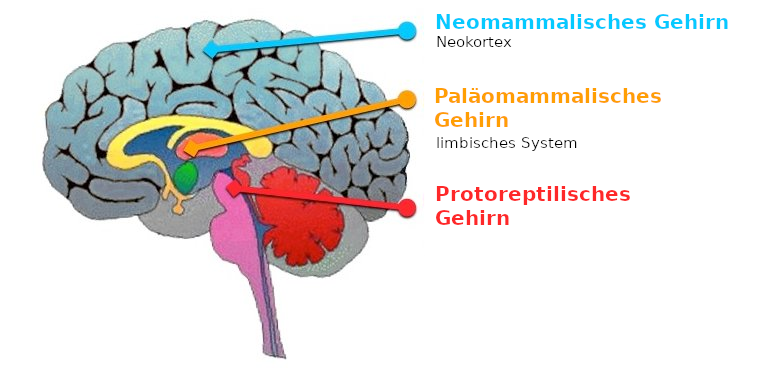
\includegraphics[width=\textwidth]{images/brain}

    \subsection{Das protoreptilische Gehirn}
    Das Reptiliengehirn ist auch als das urzeitliche Tiergehirn oder der Reptilienkomplex bekannt.
    Es befindet sich im Hirnstamm, direkt über der Stelle, an der das Rückenmark den Schädel erreicht.
    Dies ist der primitivste Teil des menschlichen Gehirns.
    Es beginnt sich bereits in der Gebärmutter zu entwickeln und beeinflusst somit alles, was Neugeborene tun (Atmen, Essen, Schlafen, Aufwachen, Weinen, Wasserlassen, Stuhlgang).
    Der Hirnstamm kontrolliert zusammen mit dem Hypothalamus die Energie des Organismus.
    Dies wird als “Homöostase” bezeichnet.
    Dieser Begriff bezieht sich auf die Aufrechterhaltung des internen Gleichgewichts.
    Die Funktionen, die das Reptiliengehirn steuert, sind grundlegender Natur.
    Wir vernachlässigen jedoch oft ihre Bedeutung, wenn wir an die fortgeschritteneren Funktionen unseres Geistes denken, beispielsweise an das abstrakte Denken.

    Viele psychische Probleme hängen mit Schwierigkeiten in den grundlegenden Funktionen zusammen, die das Reptiliengehirn aufrechterhält.
    Bei einer Traumabehandlung muss der Spezialist beispielsweise berücksichtigen, ob der Körper in ein Ungleichgewicht geraten ist.

    \subsection{Das paläomammalische Gehirn}\label{subsec:das-palaomammalische-gehirn}
    Dier Teil des Gehirns wird auch das \textit{limbische System} oder das emotionale Gehirn genannt.

    Dieses System befindet sich direkt über dem Reptiliengehirn im Zentrum des zentralen Nervensystems.
    Es beginnt von dem Moment an, sich zu entwickeln, wenn das Baby geboren wird.
    Das emotionale Gehirn ist abhängig reift mit der Erfahrung und bestimmt das Temperament des Kindes.

    Einige Autoren betrachten das emotionale Gehirn auch als Mischung aus Reptilienhirn und limbischem System.
    Einig sind sie sich darin, dass es das Zentrum unserer Emotionen und unseres Gefahrenmonitors ist.
    Demzufolge aktivieren intensive Emotionen das limbische System, insbesondere die Amygdala.
    Die Amygdala ist dafür verantwortlich, uns vor möglichen Gefahren zu warnen und verschiedene Reaktionen in Gang zu setzen:
    \begin{itemize}
        \item Sie triggert die Freisetzung von Stresshormonen.
        \item Außerdem vermittelt sie Nervosität.
        \item Sie erhöht die Herzfrequenz.
        \item Die Amygdala erhöht den Sauerstoffverbrauch und bereitet den Körper darauf vor, zu kämpfen oder zu fliehen.
    \end{itemize}

    Durch seine Tierstudien zeigte Grey, dass die Sensibilität gegenüber Stressreizen umso stärker ist, je niedriger der Serotoninspiegel ist – und umgekehrt.
    Bei männlichen Affen beobachtete er zum Beispiel, wie die Position des Individuums in der Hierarchie der Gruppe den Serotoninspiegel beeinflusste.

    Bestimmte Personen, die traumatische Ereignisse erlebt haben, registrieren zwar eine Bedrohung, doch ihr Bewusstsein verhält sich so, als ob nichts passiert wäre.
    Obwohl der Geist lernen kann, emotionale Botschaften aus dem Gehirn zu ignorieren, werden die Warnsignale des Körpers nicht unterbunden.
    Dies bedeutet, dass das emotionale Gehirn unabhängig von unserer geistigen Reaktion weiterhin funktioniert.

    Außerdem sind beide Teile des dreieinigen Gehirns (Reptiliengehirn und emotionales Gehirn) für die Aufzeichnung von Erlebnissen sowie für das Management unserer Physiologie und Identifikation (Komfort, Sicherheit, Bedrohungen, Hunger, Müdigkeit, Verlangen, Vergnügen, Schmerz) verantwortlich.

    \subsection{Das neomammalische Gehirn}\label{subsec:das-neomammalische-gehirn}
    Dies ist der jüngste Teil des dreieinigen Gehirns.
    Er ist auch als Neokortex bekannt und ist derjenige, der uns am meisten von anderen Tieren unterscheidet.
    Hier befindet sich der präfrontale Kortex, der für das Planen, Antizipieren, Erkennen von Zeit und Kontext, das Unterbinden unzulänglicher Handlungen, empathisches Verstehen usw\. zuständig ist.

    In vielen Fällen kann das rationale Gehirn das emotionale Gehirn nur dann freigeben, wenn es weiß und versteht, was mit ihm passiert ist, zum Beispiel bei einem Trauma.
    Für viele Menschen ist es einfacher, zu sagen, was passiert ist, als ihre inneren Erfahrungen wahrzunehmen, zu reflektieren und in Worte zu fassen.
    Die Stirnlappen sind Teil des rationalen Gehirns.
    Sie sind für die Regulierung von Impulsen und auch angemessenes Verhalten in einer bestimmten Situation verantwortlich.
    Eine korrekte Funktion der Stirnlappen ist entscheidend, um folgende Funktionen ausführen zu können:
    \begin{itemize}
        \item Pflege gesunder Beziehungen zu anderen Menschen.
        \item Vermeidung, Dinge zu tun, die uns gefährden könnten oder die andere Menschen verletzen könnten.
        \item Regulierung unserer Impulse, wie Hunger, Sexualtrieb, Wut
    \end{itemize}

    Das rationale Gehirn macht nur 30\% des Gesamtvolumens aus und verwaltet im Wesentlichen unsere Außenwelt.
    Das Verstehen von Vorgängen, das Erreichen von Zielen, das Verwalten der Zeit und das Sequenzieren von Aktionen sind einige seiner Hauptfunktionen.
    Darüber hinaus ist die zelluläre und biochemische Organisation des Neokortex komplexer als die des emotionalen Gehirns.


    \begin{bfhNoteBox}
        Unser Gehirn kann gemäss dem Modell des dreieinigen Gehirns in drei
    \end{bfhNoteBox}


    \section{Wie das limbische System auf das Umfeld reagiert}\label{sec:die-reaktionen-des-limbischen-systems}
    Unser limbisches System hat im Laufe der menschlichen Entwicklung, drei überlebensnotwendige Reaktionen erlernt.
Diese Reaktionen haben einen wichtigen Einfluss auf unser Verhalten in Gefahrensituationen. 
Während zu Beginn der Menscheit urzeitliche Raubtiere eine Gefahr darstellten, sind es heutzutage alltägliche Stresssituationen, in denen 
der limbische Teil unseres Gehirns diese folgenden drei alternativen Reaktionen auslöst.

\begin{itemize}
    \item Schockstarre
    \item Flucht
    \item Kampf
\end{itemize}

\subsection{Schockstarre}
Wie bereits erwähnt haben wir das limbische System von unseren Vorfahren geerbt. Da die meisten Tiere bzw.
Raubtiere auf Bewegung reagieren (da Bewegung von Beutetieren bei diesen den Jagd-Instikt auslöst), war
die erste Verteidigungsstrategie unserer Vorfahren, wie auch von den meisten Tieren, angesichts einer solchen Gefahr in die Schockstarre 
zu fallen. Den meisten ist sicherlich auch bekannt, dass sich viele Tiere sogar tot stellen, wenn sie sich bedroht fühlen,
was ein Beispiel für eine extreme Form der Schockstarre ist. 
Heutzutage ist es jedoch sehr unwahrscheinlich, dass wir in unserem Alltag Raubtieren begegnen und trotzdem
gibt es moderne Alltagssituationen, in denen wir uns plötzlich bedroht oder verunsichert fühlen, auf die wir auf viel
subtilere Weise mit Schockstarre reagieren können. 
So kann man beispielsweise oft beobachten, wie Menschen oft erstarren, wenn sie bei einer
verbotenen oder geheimen Tat ertappt werden. Ein weiteres Beispiel ist, wie wir plötzlich kurz verharren, wenn wir
merken, dass wir etwas vergessen haben. Dieser kurzer Moment der Schockstarre verschafft uns Zeit schnell darüber nachzudenken,
wie wir vorgehen wollen (wie wir auf eine Bedrohungen oder Stresssituation am Besten reagieren müssen). 


\subsection{Flucht}
In gewissen gefährlichen Situationen, kann es sein, dass die Schockstarre ungeeignet ist oder nicht ausreicht als Reaktion,
um einer Gefahr zu entkommen. Das limbische System hat für solche Fälle eine weitere Reaktion auf Bedrohungen erlernt;
die Flucht. Viele Tiere, wie auch unserer Vorfahren, mussten ohne zu Überlegen als instiktive Reaktion in gewissen Situtationen
schnellst möglich fliehen und von Bedrohungen, wie Raubtieren, davonlaufen. Da wir jedoch heutzutage
nicht mehr in der Wildnis leben, sehen moderne Bedrohungen etwas anders aus und von denen laufen wir meistens nicht weg.
Doch auch wenn die Verhaltensweise bei einer "Flucht-Reaktion" sich nicht mehr so extrem zeigt, können wir sie heute noch beobachten.
Sich von Dingen oder Personen abwenzuwenden, sich einem unangehnehmen Gespräch zu entziehen, räumlichen Abstand zu gewinnen, den Blick abzuwenden, etwas vor sich
(beispielsweise beim Sitzen auf den Schoss) zu legen, sind gute Beispiele dafür.
Mit solchen Abwehrgesten versuchen wir uns von Dingen oder Personen in Stresssituationen zu distanzieren oder abzugrenzen und diese können wir
als nonverbale Signale in einer Kommunikation beobachten.


\subsection{Kampf}
Die letzte und radikalste Reaktion vom unserem limbischem System als Überlebenstaktik ist der Kampf.
D.h. wenn alles andere nicht hilft, gehen wir über in den Angriff, dabei verwandeln wir Angst in Wut um.
Da jedoch das Ausleben von Wut als Gewalt in unserem heutigen Alltag nicht nur unangebracht sondern auch gesetzeswidrig ist,
haben wir moderne Formen entiwckelt einen "Angriff" auszuüben: Streit, Schimpfwörter, Anschuldigungen, Provokationen und ähnliches.
So kann es sein, dass Menschen "aggressiv" reagieren, wenn sie sich bedroht fühlen oder verunsichert fühlen in gewissen Stresssituationen.
Den Kampf-Zustand zeigen viele auch (bewusst oder unbewusst) auch in ihrer Körpersprache: die Körperhaltung
verändert sich, beispielsweise streckt man die Brust aus oder setzt einen strengen Blick ein. 



    \section{Definition: Nonverbale Kommunikation}
    Der Teil der Kommunikation, welchen wir oft umgangssprachlich als \textit{Körpersprache} bezeichnen, ist


    \part{Praxis}


    \section{Angewandte nonwerbale Kommunikation}

    \subsection{Wie andere nonvberbal kommunizieren}

    \subsubsection{10 Gebote zur Entschlüsselung nonverbaler Signale}
    \hskip 12pt\relax\textbf{1. Gebot: Du sollst ein aufmerksamer Beobachter deiner Umgebung sein.}
    \par\textbf{2. Gebot: Du sollst kontextbezogen beobachten.}
    \par\textbf{3. Gebot: Du sollst lernen, universell gültige nonverbale Verhaltensweisen zu erkennen.}
    \par\textbf{4. Gebot: Du sollst lernen, idiosynkratische nonverbale Verhaltensweisen zu erkennen und zu deuten.}
    \par\textbf{5. Gebot: Du sollst im Umgang mit anderen versuchen, ihr Normalverhalten zu ermitteln.}
    \par\textbf{6. Gebot: Du sollst versuchen, immer nach multiplen Tells ausschau zu halten - Verhaltensweisen, die in Kombination oder in Folge auftreten.}
    \par\textbf{7. Gebot: Du sollst nach Verhaltensänderungen Ausschau halten, die auf eine Veränderung der Gedanken, Gefühle, Interessen oder Absichten hinweisen.}
    \par\textbf{8. Gebot: Du sollst lernen, falsche oder irreführende nonverbale Signale zu erkennen.}
    \par\textbf{9. Gebot: Du sollst den Unterschied zwischen Behagen und Unbehagen erkennen.}
    \par\textbf{10. Gebot: Du sollst diskret sein, wenn du andere beobachtest.}

    \subsection{Wie wir nonvberbal kommunizieren}

    \subsubsection{Unser Verhalten}

    \subsubsection{Unser Aussehen}

    \subsubsection{Der äussere Eindruck}

    \subsubsection{Situatives nonverbalses Verhalten}

    \subsubsection{Gefühlsäusserungen}

    \subsubsection{Täuschungen}


    \begin{bfhNoteBox}
        A note box.
    \end{bfhNoteBox}

    \printbibliography


\end{document}
